\section{Three ways to describe a distribution}
\begin{frame}{Three primary representations of a distribution}

\structure{Given random variable $X$ with values in $\mR^d$, we focus on three primary ways to describe its distribution:}

\vskip 1em
\structure{1. Probability measure $P_X$}
\begin{itemize}
\item assigns probabilities to sets: $P_X(A)$ for $A \subseteq \mR^d$
\item most fundamental representation
\end{itemize}

\vskip 0.5em
\structure{2. Cumulative distribution function (CDF) $F_X$}
\begin{itemize}
\item $F_X(x) = P_X((-\infty, x])$ (for $x \in \mR^d$, component-wise)
\item always exists
\end{itemize}

\vskip 0.5em
\structure{3. Probability density function (PDF) $p_X$}
\begin{itemize}
\item when it exists: $P_X(A) = \int_A p_X(x) \, dx$
\item does not always exist!
\end{itemize}

\vskip 1em
\alert{These are three different ways to represent the same probabilistic object}

\vskip 0.5em
\structure{Note:} other representations exist (characteristic function, moment generating function, etc.) but we focus on these three

\end{frame}

\note[enumerate]
{
\item This is a key conceptual point that students often miss
\item The measure, CDF, and density (when it exists) all describe the same distribution
\item Other representations exist: characteristic function $\phi_X(t) = E[e^{itX}]$, moment generating function $M_X(t) = E[e^{tX}]$, quantile function, etc.
\item We focus on these three because: (1) measure is fundamental, (2) CDF always exists, (3) density is what we compute with in ML
\item Measure is most general, CDF always exists, density only sometimes exists
\item In ML we mostly work with densities, but need to understand when they exist
\item Component-wise for CDF in $\mR^d$: $F_X(x_1, \ldots, x_d) = P_X((-\infty, x_1] \times \cdots \times (-\infty, x_d])$
}

\begin{frame}{Interlude: integration with respect to a measure}

\structure{What you know - Riemann integration:}
\[
\int_a^b f(x) \, dx = \text{area under curve from } a \text{ to } b
\]
\begin{itemize}
\item integrate over interval $[a,b]$
\item $dx$ is infinitesimal length element
\end{itemize}

\vskip 1em
\structure{Generalization - integration w.r.t. measure $\mu$:}
\[
\int_A f \, d\mu
\]
\begin{itemize}
\item $A$ - any measurable set (not just intervals)
\item $\mu$ - measure that "weighs" different parts of space
\item $d\mu$ - infinitesimal measure element
\end{itemize}

\vskip 1em
\structure{Intuition:} sum up $f$ weighted by measure $\mu$ over set $A$

\end{frame}

\note[enumerate]
{
\item Riemann integration: only over intervals, uses length/area/volume
\item Measure integration: over any measurable set, uses any measure
\item The measure $\mu$ determines how we "weigh" different parts of the space
\item This is a generalization that will let us work with probability measures
}

\begin{frame}{Interlude: Lebesgue measure and notation}

\structure{Lebesgue measure $\lambda$ on $\mR^d$ - generalizes length/area/volume}

\vskip 0.5em
For interval $I = [a,b]$ in $\mR$: $\lambda(I) = b - a$ (length)\\
For set $A \subseteq \mR^d$: $\lambda(A) = $ volume of $A$

\vskip 1em
\structure{Integration w.r.t. Lebesgue measure:}
\[
\int_A f \, d\lambda = \int_A f(x) \, dx \quad \text{(familiar notation!)}
\]
\begin{itemize}
\item $d\lambda = dx$ is the volume element
\item recovers familiar integration notation
\end{itemize}

\vskip 1em
\structure{Notation variants (all equivalent):}
\[
\int_A f \, d\mu = \int_A f(x) \, \mu(dx) = \int_A f(x) \, d\mu(x)
\]

\vskip 0.5em
\alert{This generalizes integration to work with any measure, not just volume}

\end{frame}

\note[enumerate]
{
\item Lebesgue measure is the "natural" measure on Euclidean space
\item For nice functions on nice sets: Riemann = Lebesgue integration
\item But Lebesgue integration works for much wider class of functions and sets
\item The notation $dx$ is shorthand for $d\lambda(x)$ (Lebesgue measure)
\item Example with counting measure: $\int_A f \, d\# = \sum_{x \in A} f(x)$ (discrete sum becomes integral!)
\item Example with probability: $\int_{\mR^d} f \, dP_X = E[f(X)]$ (expectation as integral)
\item This framework unifies discrete and continuous cases
}

\begin{frame}{Probability measure - the fundamental object}

\structure{Probability measure $P_X: \mathscr{B}(\mR^d) \to [0,1]$}

\vskip 0.5em
\structure{Definition:}
\begin{itemize}
\item assigns probability to measurable sets $A \in \mathscr{B}(\mR^d)$ (Borel sets)
\item $P_X(A) = \mP(X \in A) = $ probability that $X$ takes value in $A$
\end{itemize}

\vskip 1em
\structure{Example: Gaussian $X \sim \mathcal{N}(0, 1)$ on $\mR$}
\begin{itemize}
\item $P_X([0, 1]) = \int_0^1 \frac{1}{\sqrt{2\pi}} e^{-x^2/2} \, dx \approx 0.34$
\item $P_X(\mR) = 1$
\item $P_X(\{0\}) = 0$ (single point has zero probability)
\end{itemize}

\vskip 1em
\structure{Properties:}
\begin{itemize}
\item most general representation
\item works for discrete, continuous, and mixed distributions
\item but often hard to work with directly
\end{itemize}

\end{frame}

\note[enumerate]
{
\item Borel sets are generated by open sets - think of them as "all reasonable subsets"
\item For continuous distributions, individual points have zero measure
\item Measure is the fundamental object, but we often use CDF or density for computation
\item Example calculation shows that we integrate the density to get the measure
}

\begin{frame}{Cumulative distribution function (CDF)}

\structure{CDF $F_X: \mR^d \to [0, 1]$}

\vskip 0.5em
\structure{Definition (for $\mR$):}
\[
F_X(x) = P_X((-\infty, x]) = \mP(X \leq x)
\]

\vskip 1em
\structure{Example: Gaussian $X \sim \mathcal{N}(0, 1)$}
\[
F_X(x) = \int_{-\infty}^x \frac{1}{\sqrt{2\pi}} e^{-t^2/2} \, dt = \Phi(x)
\]
\begin{itemize}
\item $F_X(0) = 0.5$ (half the probability below 0)
\item $F_X(-\infty) = 0$, $F_X(\infty) = 1$
\end{itemize}

\vskip 1em
\structure{Properties:}
\begin{itemize}
\item always exists (for any distribution)
\item non-decreasing, right-continuous
\item $P_X((a, b]) = F_X(b) - F_X(a)$
\end{itemize}

\end{frame}

\note[enumerate]
{
\item CDF is unique representation - different distributions have different CDFs
\item For multidimensional case: $F_X(x_1, \ldots, x_d) = P_X((-\infty, x_1] \times \cdots \times (-\infty, x_d])$
\item CDF can have jumps (discrete distributions) or be continuous
\item Derivative of CDF gives density (when density exists)
\item In practice: we rarely work with CDF directly in ML, but it's theoretically important
}

\begin{frame}{Probability density function (PDF)}

\structure{PDF $p_X: \mR^d \to [0, \infty)$}

\vskip 0.5em
\structure{Definition:} when it exists,
\[
P_X(A) = \int_A p_X \, d\lambda = \int_A p_X(x) \, dx
\]
where $\lambda$ is Lebesgue measure (volume)

\vskip 0.5em
\structure{Interpretation:}
\begin{itemize}
\item $p_X$ is \alert{density} - probability per unit volume
\item $P_X$ is "weighted" by density: $dP_X = p_X \, d\lambda$ or $dP_X(x) = p_X(x) \, dx$
\item $p_X = \frac{dP_X}{d\lambda}$ - Radon-Nikodym derivative
\end{itemize}

\vskip 1em
\structure{Example: Gaussian $X \sim \mathcal{N}(0, 1)$}
\[
p_X(x) = \frac{1}{\sqrt{2\pi}} e^{-x^2/2}, \quad P_X([a,b]) = \int_a^b p_X(x) \, dx
\]
note: $p_X(0) \approx 0.40$ can be $> 1$ (it's density, not probability!)

\vskip 1em
\structure{When does density exist?} $P_X$ absolutely continuous w.r.t. $\lambda$

\end{frame}

\note[enumerate]
{
\item Density is what we actually compute and optimize in ML
\item Density is NOT probability - it's probability per unit volume
\item Common mistake: thinking $p(x)$ must be $\leq 1$. Not true!
\item Radon-Nikodym theorem guarantees density exists when absolutely continuous
\item Discrete distributions (point masses) do not have densities
\item Mixed distributions (part discrete, part continuous) do not have densities
}

\begin{frame}{Relationship between the three}

\structure{How they relate:}

\vskip 0.5em
\begin{center}
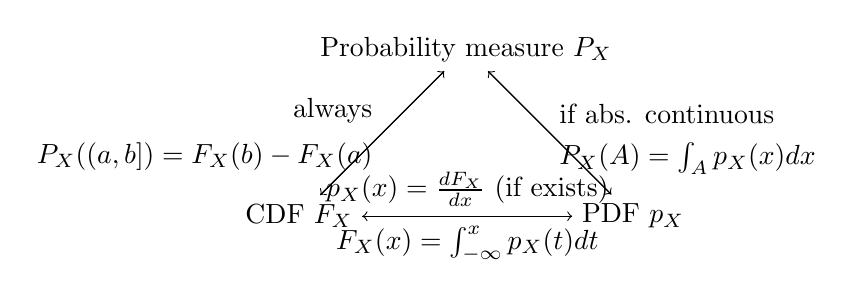
\begin{tikzpicture}[node distance=2cm]
\node (measure) {Probability measure $P_X$};
\node (cdf) [below left of=measure, node distance=3cm] {CDF $F_X$};
\node (pdf) [below right of=measure, node distance=3cm] {PDF $p_X$};

\draw[->] (measure) -- (cdf) node[midway,above left] {always};
\draw[->] (measure) -- (pdf) node[midway,above right] {if abs. continuous};
\draw[->] (pdf) -- (cdf) node[midway,below] {$F_X(x) = \int_{-\infty}^x p_X(t) dt$};
\draw[->] (cdf) -- (pdf) node[midway,above] {$p_X(x) = \frac{dF_X}{dx}$ (if exists)};
\draw[->] (pdf) -- (measure) node[midway,below right] {$P_X(A) = \int_A p_X(x) dx$};
\draw[->] (cdf) -- (measure) node[midway,below left] {$P_X((a,b]) = F_X(b) - F_X(a)$};
\end{tikzpicture}
\end{center}

\vskip 1em
\structure{Key points:}
\begin{itemize}
\item measure $\to$ CDF: always possible
\item measure $\to$ PDF: only when absolutely continuous
\item in ML: we almost always work with PDFs (assume absolute continuity)
\end{itemize}

\end{frame}

\note[enumerate]
{
\item This diagram shows all the relationships
\item Most fundamental: measure
\item Most general representation that always exists: CDF
\item Most convenient for computation: PDF (when it exists)
\item In deep learning: we assume our distributions have densities
\item This is reasonable for continuous distributions on $\mR^d$
}

\begin{frame}{Examples: discrete, continuous, mixed}

\structure{Discrete: $X \in \{0, 1, 2\}$ with $P_X(\{k\}) = 1/3$}
\begin{itemize}
\item measure: $P_X(\{0\}) = P_X(\{1\}) = P_X(\{2\}) = 1/3$
\item CDF: $F_X(x) = \begin{cases} 0 & x < 0 \\ 1/3 & 0 \leq x < 1 \\ 2/3 & 1 \leq x < 2 \\ 1 & x \geq 2 \end{cases}$ (step function)
\item PDF: \alert{does not exist} (point masses)
\end{itemize}

\vskip 1em
\structure{Continuous: $X \sim \mathcal{N}(0, 1)$}
\begin{itemize}
\item measure: $P_X(A) = \int_A \frac{1}{\sqrt{2\pi}} e^{-x^2/2} dx$
\item CDF: $F_X(x) = \Phi(x)$ (smooth, no jumps)
\item PDF: $p_X(x) = \frac{1}{\sqrt{2\pi}} e^{-x^2/2}$ \alert{exists}
\end{itemize}

\vskip 0.5em
\structure{Mixed: half point mass at 0, half uniform on $[0,1]$}
\begin{itemize}
\item PDF: \alert{does not exist} (has point mass at 0)
\end{itemize}

\end{frame}

\note[enumerate]
{
\item These examples show when density exists and when it doesn't
\item Discrete: CDF has jumps, no density
\item Continuous: CDF is smooth, density exists
\item Mixed: combination, no density
\item In generative modeling: we work with continuous distributions, so densities exist
\item Point masses and discrete distributions don't have densities w.r.t. Lebesgue measure
}
